\documentclass{article}
\usepackage[utf8]{inputenc}
\usepackage[includeheadfoot, margin=1em,headheight=2em]{geometry}
\usepackage{titling}
\geometry{a4paper, left=2cm, right=2cm, top=2cm, bottom=2cm}
\usepackage{graphicx}
\usepackage{float}
\providecommand{\versionnumber}{1.0.0}
\usepackage{enumitem}
\usepackage{array}
\usepackage[italian]{babel}
\newcolumntype{P}[1]{>{\centering\arraybackslash}p{#1}}
\renewcommand{\arraystretch}{1.5} % Default value: 1
\setlength{\droptitle}{-6em}

%font
\usepackage[defaultfam,tabular,lining]{montserrat}
\usepackage[T1]{fontenc}
\renewcommand*\oldstylenums[1]{{\fontfamily{Montserrat-TOsF}\selectfont #1}}

%custom bold 
\usepackage[outline]{contour}
\usepackage{xcolor}
\newcommand{\custombold}{\contour{black}}

%table colors
\usepackage{color, colortbl}
\definecolor{Blue}{rgb}{0.51,0.68,0.79}
\definecolor{LightBlue}{rgb}{0.82,0.87,0.90}
\definecolor{LighterBlue}{rgb}{0.93,0.95,0.96}

%Header
\usepackage{fancyhdr, xcolor}
\pagestyle{fancy}
\let\oldheadrule\headrule% Copy \headrule into \oldheadrule
\renewcommand{\headrule}{\color{Blue}\oldheadrule}% Add colour to \headrule
\renewcommand{\headrulewidth}{0.2em}
\fancyhead[L]{Analisi Celonis}
\fancyhead[C]{Samuele Vignotto}
\fancyhead[R]{
\includegraphics[height=1cm]{Logo/Y_LOGO-SOLO.png}}
\setcounter{secnumdepth}{0}

\title{\Huge{\textbf{Analisi della piattaforma di process mining Celonis}}\vspace{-1em}}
\author{Samuele Vignotto}
\date{}
\begin{document}
\maketitle
\begin{figure}[h]
  \centering
  
\includegraphics[width=6cm, height=6cm]{Logo/Y_LOGO-SOLO.png}
  \label{fig:immagine}
\end{figure}

\newpage
\tableofcontents
\newpage

\section{Introduzione}

Il process mining è una disciplina emergente che combina tecniche di data mining e di analisi dei processi aziendali per fornire una visione approfondita dei processi operativi di un'organizzazione. Una delle piattaforme leader in questo campo è Celonis, una soluzione di process mining avanzata che permette alle aziende di ottimizzare e migliorare continuamente i propri processi aziendali.

\subsection{Estrazione Automatica dei Dati}

Celonis si distingue per la sua capacità di estrarre automaticamente dati da vari sistemi informatici aziendali, tra cui ERP (Enterprise Resource Planning), CRM (Customer Relationship Management) e altri sistemi transazionali. Utilizzando queste informazioni, Celonis crea una rappresentazione visiva e dettagliata dei processi aziendali reali, consentendo agli utenti di identificare inefficienze, colli di bottiglia e deviazioni dai processi standard.

\subsection{Analisi in Tempo Reale}

Una delle funzionalità chiave di Celonis è la sua capacità di fornire un'analisi in tempo reale. Questa caratteristica permette alle organizzazioni di monitorare i propri processi in modo continuo, rilevando e risolvendo problemi immediatamente. Inoltre, Celonis offre potenti strumenti di visualizzazione che permettono agli utenti di esplorare i dati da diverse prospettive, identificando facilmente le aree critiche che necessitano di miglioramenti.

\subsection{Benchmarking}

Un altro aspetto fondamentale di Celonis è la sua funzione di benchmarking, che consente alle aziende di confrontare le proprie prestazioni con quelle di altre organizzazioni o con standard di settore. Questo confronto aiuta a identificare le migliori pratiche e a impostare obiettivi di miglioramento realistici.

\subsection{Integrazione con Machine Learning e Intelligenza Artificiale}

Celonis supporta anche l'integrazione con tecniche di machine learning e intelligenza artificiale, permettendo di prevedere l'andamento dei processi e di suggerire azioni correttive proattive. Questo approccio predittivo è particolarmente utile per anticipare problemi potenziali e mitigare rischi operativi.

\subsection{Automazione dei Processi}

Inoltre, Celonis offre funzionalità di automazione dei processi, che permettono di implementare rapidamente miglioramenti identificati attraverso il process mining. Questo porta a una riduzione dei tempi di ciclo, a una maggiore conformità e a un miglioramento generale dell'efficienza operativa.


\section{Integrazione dei dati}
I dati che la piattaforma Celonis utilizza sono catturati dagli strumenti e dai sistemi aziendali (definiti come sistemi sorgente). Questi sistemi sorgente possono essere integrati con la piattaforma Celonis, permettendo di estrarre i dati rilevanti, trasformarli secondo le esigenze e di caricarli in un modello di dati per essere utilizzati in tutta la piattaforma.

\begin{figure}[H]
    \centering
    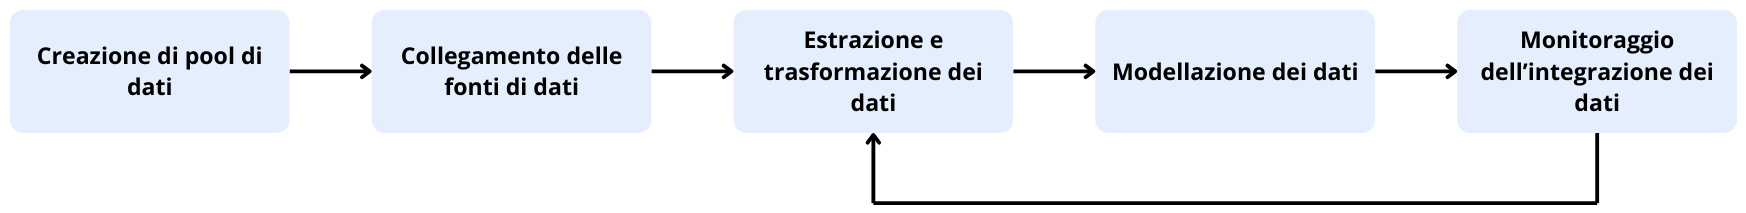
\includegraphics[width=\textwidth]{imgCelonis/IntegrazioneDati.png}
    \caption{Flusso dell'integrazione dati in Celonis}
    \label{fig:flusso-integrazione-dati-celonis}
\end{figure}

\subsection{Creazione e manutenzione di pool di dati}
Un pool di dati è l'elemento strutturale principale del flusso di lavoro di integrazione dei dati. Serve da contenitore per le fonti di dati e facilita il monitoraggio dei dati.

\subsubsection{Tipi di dati necessari}
La piattaforma richiede vari tipi di dati, tra cui file di log degli eventi, fogli di calcolo (Google Sheets, CSV, XLSX), flussi di eventi estensibili (XES) e dati da applicazioni enterprise come SAP, Oracle EBS, Salesforce, e ServiceNow. Inoltre, supporta fonti di dati cloud e database tradizionali come Microsoft SQL, Oracle e Snowflake. L'integrazione con queste fonti è facilitata da connettori specifici e dall'utilizzo di API.\\
Celonis offre connettori specifici per Oracle Database, che consentono l'estrazione dei dati direttamente dalle tabelle e dalle viste, garantendo la coerenza e l'aggiornamento continuo delle informazioni. Questo processo include la gestione di schemi complessi e l'ottimizzazione delle query per ridurre l'impatto sulle prestazioni del database di origine.\\
Per quanto riguarda i sistemi ERP, Celonis supporta l'integrazione con soluzioni come SAP e Oracle E-Business Suite. L'estrazione dei dati da questi sistemi prevede l'utilizzo di API e connettori dedicati, che facilitano la raccolta di dati transazionali e master. Questo consente di ottenere una visione completa dei processi aziendali, dalla gestione degli ordini alla supply chain, migliorando così l'analisi e l'ottimizzazione dei processi.

\subsubsection{Vantaggi della piattaforma}
Uno dei principali vantaggi di Celonis è la sua capacità di connettersi a una vasta gamma di fonti di dati, sia on-premise che cloud, offrendo molta flessibilità. La piattaforma permette l'estrazione in tempo reale dei dati, garantendo che le analisi siano sempre basate su informazioni aggiornate. Inoltre, Celonis supporta la trasformazione dei dati con strumenti integrati, semplificando il processo di preparazione dei dati per l'analisi.

\subsubsection{Svantaggi della Piattaforma}
L'integrazione dei dati in Celonis può presentare alcune sfide. L'aggiornamento e la manutenzione delle connessioni ai vari sistemi possono risultare complessi, soprattutto in ambienti IT eterogenei. Infine, l'uso intensivo di risorse durante i processi di estrazione e trasformazione può influire sulle prestazioni dei sistemi coinvolti.

\section{Business miner}
Business Miner di Celonis è un'applicazione progettata per aiutare le aziende a scoprire, analizzare e ottimizzare i loro processi aziendali. Utilizzando la tecnologia avanzata di process mining, Business Miner permette di esaminare i dati operativi, identificare inefficienze e proporre soluzioni basate su dati concreti.\\
Attraverso un'interfaccia intuitiva e user-friendly, gli utenti possono visualizzare mappature precise dei flussi di lavoro, individuare colli di bottiglia, e monitorare le prestazioni.\\
Una delle caratteristiche distintive di Business Miner è la sua capacità di fornire insights immediati grazie all'intelligenza artificiale e agli algoritmi di machine learning. Questi strumenti analizzano grandi volumi di dati per individuare pattern e tendenze nascoste, suggerendo modifiche operative che possono portare a significativi miglioramenti in termini di efficienza e produttività.\\
L'applicazione offre funzionalità di reportistica avanzata, che consentono di creare report personalizzati e dashboard interattive, facilitando la condivisione di informazioni e la presa di decisioni informate. La sua flessibilità e scalabilità la rendono adatta a organizzazioni di diverse dimensioni e settori.\\

\section{Implementazioni pratiche di Business Miner: simulazioni}

\subsection{Prima simulazione}
\subsubsection{Struttura del file CSV}
Il file CSV con i dati simulati contiene informazioni riguardanti le attività di una ditta che riceve prodotti da un'azienda, li vende online e li spedisce ai clienti. La struttura del file è la seguente:
\begin{itemize}
    \item \custombold{activity\_id}: identificativo univoco per ogni attività;
    \item \custombold{activity}: nome dell'attività svolta;
    \item \custombold{timestamp}: data e ora in cui l'attività è stata svolta;
    \item \custombold{product\_id}: identificativo del prodotto coinvolto nell'attività.
\end{itemize}
Esempio di contenuto del file CSV:
\begin{table}[htbp]
    \centering
    \begin{tabular}{|c|c|c|c|}
        \hline
        \textbf{activity\_id} & \textbf{activity} & \textbf{timestamp} & \textbf{product\_id} \\
        \hline
        1 & Receive Goods & 2023-08-02 18:20:10.465195 & 1 \\
        \hline
        2 & Quality Check & 2023-12-03 13:30:22.465195 & 1 \\
        \hline
        3 & Store in Warehouse & 2024-03-09 18:03:55.465195 & 1 \\
        \hline
        4 & Pick for Order & 2024-03-15 02:03:15.465195 & 1 \\
        \hline
        5 & Order Cancellation & 2024-05-29 08:01:26.465195 & 1 \\
        \hline
    \end{tabular}
    \caption{Activity Log}
    \label{tab:activity_log}
\end{table}
\subsubsection{Regole di simulazione dei dati}
I dati simulati sono stati generati seguendo determinate regole per garantire la coerenza temporale e la rappresentazione realistica dei processi aziendali. Le regole principali sono:
\begin{itemize}
    \item \custombold{Coerenza dei Timestamps}: I timestamp delle attività devono essere coerenti. Ad esempio, il timestamp della spedizione al cliente non può essere precedente al timestamp dell'ordine.
    \item \custombold{Cicli di attività possibili}:
    \begin{itemize}
        \item \custombold{Ciclo 1}: Receive Goods -> Quality Check -> Store in Warehouse
        \item \custombold{Ciclo 2}: Receive Goods -> Quality Check -> Store in Warehouse -> Pick for Order -> Order Cancellation
        \item \custombold{Ciclo 3}: Receive Goods -> Quality Check -> Store in Warehouse -> Pick for Order -> Receive Payment -> Pack for Shipment -> Ship to Customer -> Customer Receive Goods
        \item \custombold{Ciclo 4}: Receive Goods -> Quality Check -> Store in Warehouse -> Pick for Order -> Receive Payment -> Pack for Shipment -> Ship to Customer -> Customer Receive Goods -> Customer Feedback
        \item \custombold{Ciclo 5}: Receive Goods -> Quality Check -> Store in Warehouse -> Pick for Order -> Receive Payment -> Pack for Shipment -> Ship to Customer -> Customer Receive Goods -> Customer Feedback -> Return Processing
    \end{itemize}
\end{itemize}
\subsubsection{Analisi delle attività}
Le attività principali e la loro frequenza nei dati simulati sono le seguenti:
\begin{itemize}
    \item \custombold{Receive Goods}: 100\% dei casi;
    \item \custombold{Quality Check}: 100\% dei casi;
    \item \custombold{Store in Warehouse}: 100\% dei casi;
    \item \custombold{Pick for Order}: 84\% dei casi;
    \item \custombold{Customer Receive Goods}: 68\% dei casi;
    \item \custombold{Pack for Shipment}: 68\% dei casi;
    \item \custombold{Receive Payment}: 68\% dei casi;
    \item \custombold{Ship to Customer}: 68\% dei casi;
    \item \custombold{Customer Feedback}: 41\% dei casi;
    \item \custombold{Return Processing}: 31\% dei casi;
\end{itemize}
\subsubsection{Analisi del processo}
Il file CSV è stato utilizzato per testare diverse funzionalità della piattaforma Celonis, fornendo una visione chiara del flusso di lavoro aziendale e delle sue inefficienze.\\
Inizialmente, abbiamo esplorato la funzione "What does your process look like?", analizzando un totale di 100 casi distribuiti tra luglio 2023 e luglio 2024. Questa analisi ci ha permesso di osservare la variazione mensile dei casi, evidenziando come questi siano distribuiti lungo l'anno. Inoltre, sono stati identificati 11 processi distinti, con frequenze specifiche per ciascuna attività all'interno del processo.\\
\begin{figure}[H]
    \centering
    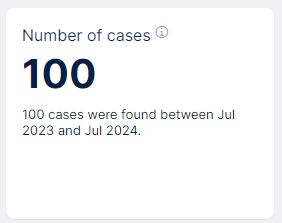
\includegraphics[width=0.33\textwidth]{imgCelonis/PrimaSimulazione/NumeroCasi.png}
    \caption{Numero di casi identificati da Celonis}
    \label{fig:Casi-Identificati_Celonis}
\end{figure}
\begin{figure}[H]
    \centering
    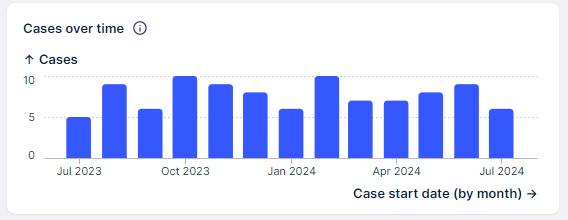
\includegraphics[width=0.33\textwidth]{imgCelonis/PrimaSimulazione/DistribuzioneCasiMesi.png}
    \caption{Distribuzione dei casi identificata da Celonis}
    \label{fig:Distribuzione-Casi_Celonis}
\end{figure}
\begin{figure}[H]
    \centering
    \includegraphics[width=0.33\textwidth]{imgCelonis/PrimaSimulazione/NumeroAttività.png}
    \caption{Numero di attività identificate da Celonis}
    \label{fig:Attività-Identificate-Celonis}
\end{figure}
La visualizzazione grafica generata da Celonis ha mostrato chiaramente le sequenze delle attività, permettendoci di comprendere meglio il flusso dei processi aziendali. I filtri disponibili ci hanno consentito di personalizzare la visualizzazione, focalizzandoci su dettagli specifici dei casi e delle attività.\\
\begin{figure}[H]
    \centering
    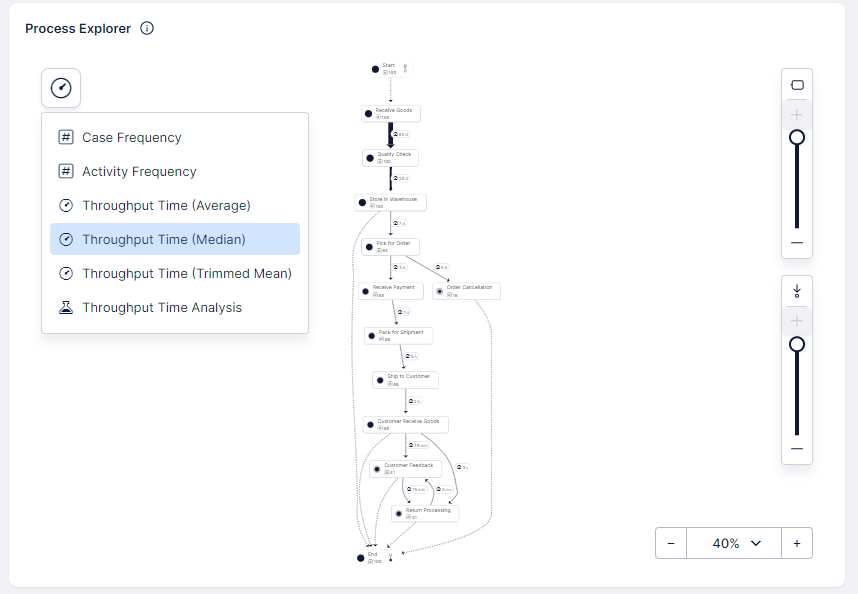
\includegraphics[width=\textwidth]{imgCelonis/PrimaSimulazione/GrafoSimulazione.png}
    \caption{Grafo del processo creato da Celonis}
    \label{fig:Grafo-processo_Celonis}
\end{figure}
Passando alla sezione "How long does your process take?", abbiamo esaminato i tempi di esecuzione delle attività dall'inizio alla fine del processo, fornendo una chiara distribuzione temporale dei casi. Questa analisi ha permesso di identificare le connessioni con ampie distribuzioni di Throughput Times, rivelando inefficienze significative.\\
\begin{figure}[H]
    \centering
    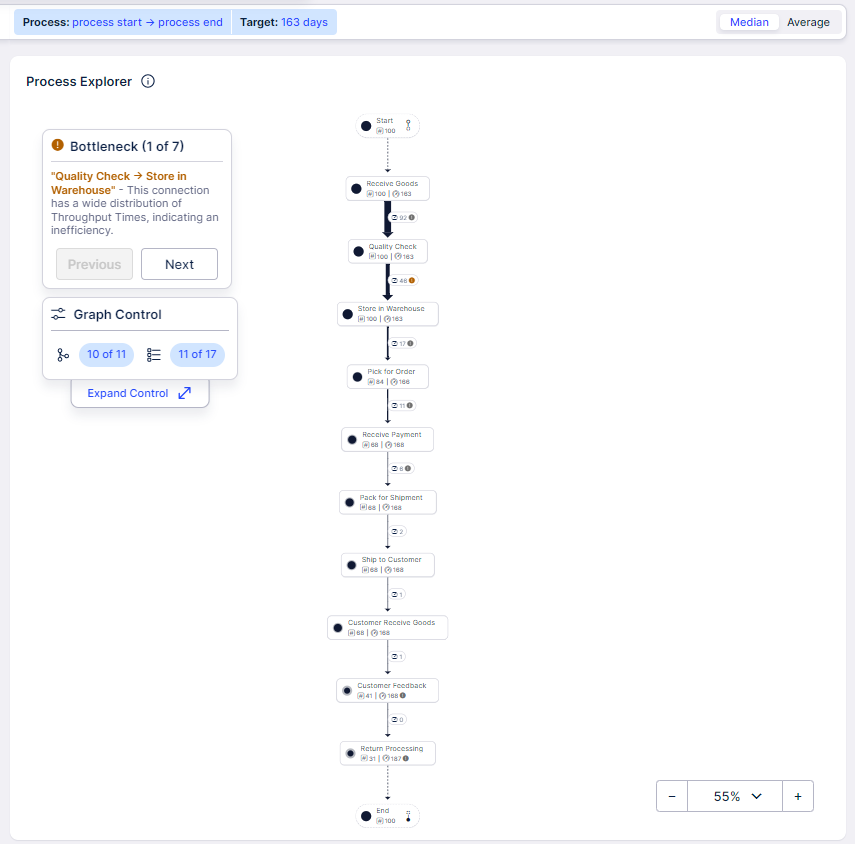
\includegraphics[width=\textwidth]{imgCelonis/PrimaSimulazione/GrafoColliDiBottiglia.png}
    \caption{Grafo del processo con evidenziati i colli di bottiglia}
    \label{fig:Grafo-colli-di-bottiglia}
\end{figure}
Celonis ha identificato vari colli di bottiglia nei dati simulati. Tra questi, la connessione tra Quality Check e Store in Warehouse ha mostrato una distribuzione ampia dei tempi di esecuzione, indicando un'inefficienza. Analoghe osservazioni sono state fatte per le connessioni tra Receive Goods e Quality Check, Store in Warehouse e Pick for Order, Receive Payment e Pack for Shipment, Pick for Order e Receive Payment. Inoltre, le attività di Customer Feedback e Return Processing hanno mostrato tempi di esecuzione elevati, contribuendo ulteriormente alle inefficienze del processo.\\
\begin{figure}[H]
    \centering
    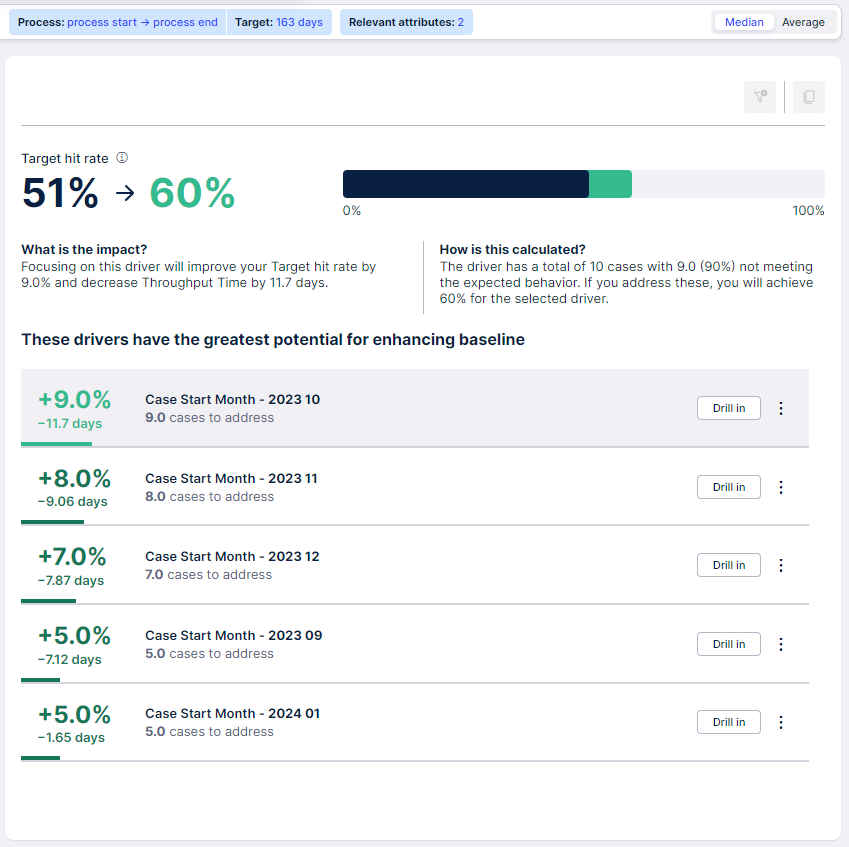
\includegraphics[width=\textwidth]{imgCelonis/PrimaSimulazione/MiglioramentiSuggeriti.png}
    \caption{Miglioramenti suggeriti da Celonis}
    \label{fig:Miglioramenti-suggeriti}
\end{figure}
Questa analisi approfondita ha evidenziato come Celonis possa identificare i punti deboli nei processi aziendali e suggerire miglioramenti concreti, contribuendo a ottimizzare l'efficienza operativa complessiva.
\subsubsection{Conclusioni}
Il file con i dati simulati ha permesso di testare efficacemente le funzionalità del modulo Business Miner di Celonis. La piattaforma si è dimostrata capace di fornire una visione dettagliata dei processi aziendali, identificare inefficienze e suggerire miglioramenti concreti. Le analisi eseguite hanno evidenziato come Celonis possa essere utilizzato per analisi più complesse e realistiche, offrendo un potente supporto per l'ottimizzazione dei processi aziendali.

\subsection{Seconda simulazione}
Il file CSV è stato creato mediante uno script Python che simula una serie di attività relative alla produzione e alla gestione degli ordini di prodotti. Inoltre, per la simulazione dei dati, sono stati presi in considerazione anche i dati estratti manualmente da un database di un sistema gestionale.
\subsubsection{Regole di simulazione dei dati}
\custombold{Impostazione delle date iniziali}\\
Ogni ciclo di attività inizia con la prima attività programmata tra il 1 gennaio 2019 e il 31 dicembre 2020.\\
\custombold{Definizione delle tipologie di prodotti}\\
Viene creata una lista di 30 tipi di scarpe, denominate "Scarpe tipo 1" fino a "Scarpe tipo 30".\\
\custombold{Definizione delle attività e delle durate}\\
Sono state definite 17 attività, ciascuna con un ID unico e una durata variabile. Le durate delle attività sono espresse in minuti o giorni, a seconda dell'attività specifica.\\
\custombold{Generazione di un ciclo di attività per prodotto}\\
Per ciascun prodotto, viene generato un ciclo di attività che segue le seguenti regole:
\begin{itemize}
    \item \custombold{attività obbligatorie}: alcune attività avvengono in un ordine fisso. Ad esempio, "COnferma ordine" è sempre seguita da "Creazione progetto";
    \item \custombold{modifica del progetto}: un numero casuale di modifiche al progetto (da 1 a 5) può essere aggiunto dopo la creazione del progetto;
    \item \custombold{gestione degli ordini fornitore}: un numero casuale (da 1 a 3) di cicli di gestione ordini fornitore può essere inserito, ognuno dei quali può includere attività come "Ordine fornitore", "Arrivo offerta fornitore", "Ordine annullato", o "Ordine sospeso";
    \item \custombold{produzione}: vengono aggiunte attività relative alla produzione, come "Stampa scheda di produzione", "Inizio ciclo di produzione" e "Termine ordine di produzione";
    \item \custombold{fatturazione e consegna}: dopo la produzione, vengono aggiunte le attività di "Invio fattura cliente" e "Consegna". La ricezione del pagamento della fattura può avvenire in modo casuale prima o dopo la consegna, ma deve avvenire almeno una volta per ciclo.
\end{itemize}
\custombold{Generazione dei timestamp}\\
Ogni attività riceve un timestamp generato casualmente basato su un intervallo di tempo definito per quella specifica attività.\\
\custombold{Ciclo di generazione dei dati}\\
Il numero di prodotti varia tra 300 e 500, determinato casualmente. Per ogni prodotto, viene generato un ciclo di attività completo, assicurandosi che tutte le attività obbligatorie siano inserite nel corretto ordine e che le attività casuali siano distribuite come specificato.
\subsubsection{Monitoraggio del rispetto delle scadenze}
La funzionalità di monitoraggio del rispetto delle scadenze di Celonis consente di capire se le varie attività del processo vengono completate entro i tempi prestabiliti, identificando eventuali ritardi e le loro cause principali.\\
\custombold{Configurazione}\\
La puntualità viene definita in base a due input: un'attività di completamento e un'attività di scadenza. Ad esempio, un ordine è considerato completato in tempo se l'attività di Registrazione Emissione Merci si verifica prima dell'attività di Scadenza Superata. Si tiene anche conto di un periodo di tolleranza.\\
\begin{figure}[H]
    \centering
    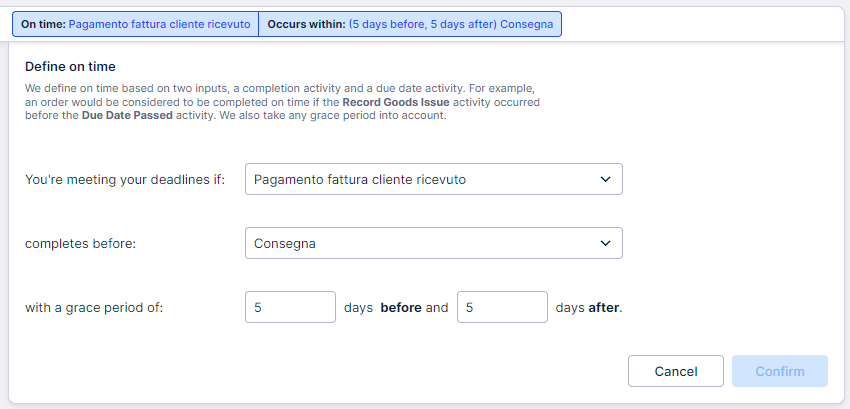
\includegraphics[width=\textwidth]{imgCelonis/SecondaSimulazione/configurazione-meeting-deadlines.png}
    \caption{Schermata di configurazione del monitoraggio del rispetto delle scadenze}
    \label{fig:configurazione-meeting-deadlines}
\end{figure}
\custombold{Campi di configurazione}\\
\begin{itemize}
    \item \custombold{you're meeting your deadlines if}: qui è selezionata l'attività "Pagamento fattura cliente ricevuto". Questo indica che la scadenza viene rispettata se questa attività è completata entro il periodo definito;
    \item \custombold{completes before}:  qui è selezionata l'attività "Consegna". Questo campo definisce che l'attività "Pagamento fattura cliente ricevuto" deve essere completata prima della "Consegna" per essere considerata in tempo.
    \item \custombold{with a grace period of}: qui vengono definiti i periodi di tolleranza: \begin{itemize}
        \item \custombold{5 days before}: un periodo di 5 giorni prima della data di consegna è accettabile.
        \item \custombold{5 days after}: un periodo di 5 giorni dopo la data di consegna è anch'esso accettabile.
    \end{itemize}
\end{itemize}
\custombold{On-Time rate e grafico del tasso di puntualità nel tempo}\\
Questa schermata fornisce una panoramica dettagliata delle prestazioni in termini di rispetto delle scadenze per un determinato processo.\\
\begin{figure}[H]
    \centering
    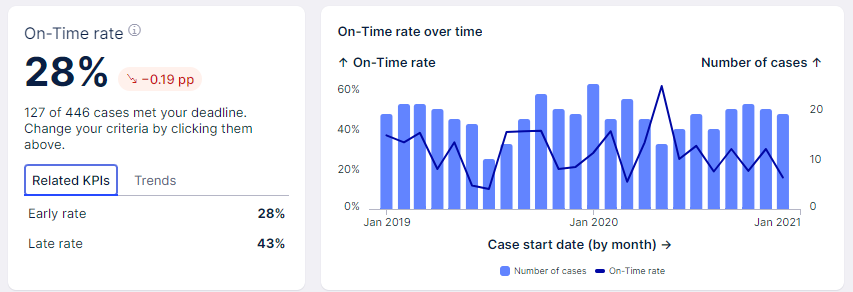
\includegraphics[width=\textwidth]{imgCelonis/SecondaSimulazione/On-Time-rate-grafico-tasso-puntualita.png}
    \caption{Schermata di monitoraggio del tasso di puntualità}
    \label{fig:monitoraggio-on-time-rate}
\end{figure}
\custombold{On-Time rate}\\
La percentuale di casi che hanno rispettato la scadenza. Attualmente è del 28\%, indicando che solo il 28\% delle attività analizzate è stato completato entro il periodo di tolleranza definito.\\
\begin{itemize}
    \item \custombold{127 of 446 cases met your deadline}: questo significa che 127 casi su 446 totali hanno rispettato la scadenza;
    \item \custombold{indicatori di performance collegati}:\begin{itemize}
        \item \custombold{early rate}: la percentuale di casi completati in anticipo rispetto alla scadenza, che è del 28\%;
        \item \custombold{late rate}: la percentuale di casi completati in ritardo rispetto alla scadenza, che è del 43\%.
    \end{itemize}
\end{itemize}
\custombold{Grafico del tasso di puntualità nel tempo}\\
Il grafico mostra l'andamento del tasso di puntualità nel tempo, rappresentando i dati mese per mese.\\
\begin{itemize}
    \item \custombold{Asse Y sinistro (On-Time rate)}: rappresenta la percentuale di attività completate in tempo;
    \item \custombold{asse y destro (Number of cases)}: rappresenta il numero di casi analizzati per ogni mese;
    \item \custombold{barre azzurre}: indicano il numero di casi per ciascun mese;
    \item \custombold{linea blu}: indica il tasso di puntualità per ciascun mese.
\end{itemize}
\custombold{Analisi e interpretazione}\\
Il grafico mostra fluttuazioni nel tasso di puntualità nel tempo. Ci sono picchi e cali evidenti, suggerendo che la performance nel rispetto delle scadenze varia notevolmente di mese in mese.\\
Con un on-time rate del 28\%, si evidenzia un problema significativo nel rispetto delle scadenze, dato che una grande percentuale di attività (72\%) non è stata completata entro i tempi stabiliti.\\
\custombold{Dettagli specifici}:
\begin{itemize}
    \item la \custombold{percentuale di completamento anticipato} (28\%) è la stessa della percentuale di attività completate in tempo, indicando che un numero significativo di attività viene completato molto prima della scadenza.
    \item la \custombold{percentuale di completamento in ritardo} (43\%) è piuttosto alta, suggerendo che quasi la metà delle attività non viene completata entro i tempi previsti.
\end{itemize}

\custombold{On-Time breakdown}\\
Questa tabella offre una suddivisione dettagliata del tasso di puntualità per mese di inizio dei casi analizzati.\\
\begin{figure}[H]
    \centering
    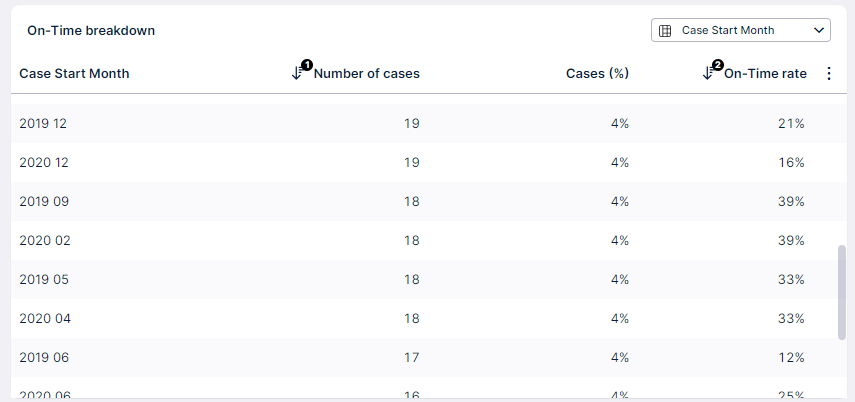
\includegraphics[width=\textwidth]{imgCelonis/SecondaSimulazione/on-time-breakdown.png}
    \caption{Tabella di monitoraggio del tasso di puntualità per mese}
    \label{fig:tabella-on-time-breakdown}
\end{figure}
\custombold{Intestazione delle colonne}
\begin{itemize}
    \item \custombold{case start month}: mese di inizio dei casi analizzati;
    \item \custombold{number of cases}: numero di casi iniziati in quel mese specifico;
    \item \custombold{cases(\%)}: percentuale dei casi rispetto al totale analizzato;
    \item \custombold{on-time rate}: percentuale di casi completati entro le scadenze per ogni mese.
\end{itemize}
\custombold{Interpretazione della tabella}\\
La tabella offre una visione chiara della puntualità dei casi analizzati per ogni mese. Permette di identificare i mesi con migliori o peggiori performance in termini di rispetto delle scadenze. Ad esempio, settembre 2019 e febbraio 2020 hanno un on-time rate del 39\%, indicando che in quei mesi una percentuale significativa dei casi è stata completata entro le scadenze.\\
D'altra parte, mesi come giugno 2019 e dicembre 2020 hanno tassi di puntualità più bassi, rispettivamente del 12\% e del 16\%, segnalando periodi in cui è stato più difficile rispettare le scadenze. Questi dati sono utili per comprendere le variazioni nella performance e per identificare le cause potenziali di ritardi in specifici periodi.\\

\custombold{On-Time behavior}\\
Il grafico rappresenta il comportamento delle attività in relazione alle scadenze.\\
\begin{figure}[H]
    \centering
    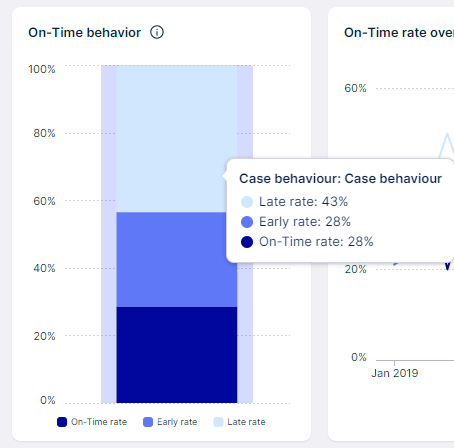
\includegraphics[width=\textwidth]{imgCelonis/SecondaSimulazione/on-time-behavior.png}
    \caption{Grafico comportamento delle attività in relazione alle scadenze}
    \label{fig:grafico-on-time-behavior}
\end{figure}
\custombold{Barre del grafico}\\
Il grafico è costituito da una barra suddivisa in tre sezioni di colori diversi, ciascuna rappresentante una diversa categoria di comportamento delle scadenze:
\begin{itemize}
    \item \custombold{blu scuro}: rappresenta la percentuale di attività completate in tempo ("On-Time rate");
    \item \custombold{blu}: rappresenta la percentuale di attività completate in anticipo ("Early rate");
    \item \custombold{azzurro}: rappresenta la percentuale di attività completate in ritardo ("Late rate").
\end{itemize}
\custombold{Dati specifici}
\begin{itemize}
    \item \custombold{On-Time rate (28\%)}: percentuale di attività completate entro le scadenze stabilite è del 28\%;
    \item \custombold{Early rate (28\%)}: percentuale di attività completate in anticipo rispetto alle scadenze è del 28\%;
    \item \custombold{Late rate (43\%)}: percentuale di attività completate in ritardo rispetto alle scadenze è del 43\%;
\end{itemize}
\custombold{Interpretazione del grafico}\\
Il grafico offre una rappresentazione chiara e sintetica del comportamento delle attività rispetto alle scadenze. La sua suddivisione in tre sezioni permette di comprendere rapidamente come le attività si distribuiscono tra completamento puntuale, anticipato e ritardato.\\
Un elemento significativo emerso dall'analisi è l'elevato tasso di ritardo: ben il 43\% delle attività viene completato oltre la scadenza, segnalando un problema rilevante nel rispetto dei tempi previsti. Questo dato indica che quasi la metà delle attività non riesce a essere conclusa entro i termini stabiliti.\\
D'altro canto, le percentuali di puntualità e di completamento anticipato risultano identiche, entrambe al 28\%. Questo significa che un numero analogo di attività viene concluso esattamente nei tempi previsti o addirittura in anticipo, mostrando una certa capacità di gestione efficace, pur evidenziando la necessità di miglioramenti nel rispetto delle scadenze.\\

\custombold{On-Time rate over time}\\
Il grafico rappresenta l'andamento del tasso di puntualità delle attività nel tempo, mese per mese.\\
\begin{figure}[H]
    \centering
    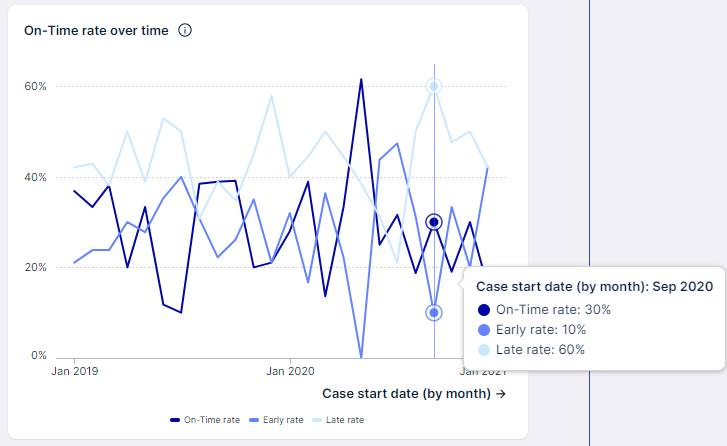
\includegraphics[width=\textwidth]{imgCelonis/SecondaSimulazione/on-time-rate-over-time.png}
    \caption{Grafico del tasso di puntualità delle attività nel tempo}
    \label{fig:grafico-on-time-rate-over-time}
\end{figure}
\custombold{Assi del grafico}
\begin{itemize}
    \item \custombold{Asse X (case start by month)}: rappresenta i mesi di inizio dei casi;
    \item \custombold{asse Y (percentuale)}: rappresenta la percentuale di casi completati, suddivisa in tre categorie: in tempo, in anticipo e in ritardo.
\end{itemize}
\custombold{Linee del grafico}
\begin{itemize}
    \item \custombold{Linea blu scuro (On-Time rate)}: indica la percentuale di casi completati in tempo per ogni mese;
    \item \custombold{linea blu (Early rate)}: indica la percentuale di casi completati in anticipo per ogni mese;
    \item \custombold{linea azzurra (Late rate}: indica la percentuale di casi completati in ritardo per ogni mese.
\end{itemize}
\custombold{Analisi e interpretazione}\\
Il grafico offre una visualizzazione dettagliata e dinamica del tasso di puntualità, dell'anticipo e del ritardo nel tempo. Analizzandolo, è possibile osservare vari trend e fluttuazioni nei tassi di completamento delle attività.\\
In particolare, si notano variazioni significative nel tasso di puntualità tra i vari mesi, con alcuni periodi caratterizzati da picchi e altri da cali evidenti. Ad esempio, a settembre 2020, il tasso di puntualità è del 30\%, un valore relativamente basso rispetto ad altri periodi.\\
Sempre a settembre 2020, si registra un elevato tasso di ritardo, con il 60\% delle attività completate oltre la scadenza, suggerendo un problema significativo in quel periodo specifico. Questo alto tasso di ritardo richiede un'analisi approfondita per identificare le cause e implementare azioni correttive.\\
Infine, il tasso di completamento anticipato a settembre 2020 è solo del 10\%, indicando che poche attività sono state completate prima delle scadenze.\\

\custombold{On-Time distribution}\\
Questo grafico rappresenta la distribuzione dei casi in base al loro completamento rispetto alle scadenze, suddivisi per giorni di anticipo o ritardo.\\
\begin{figure}[H]
    \centering
    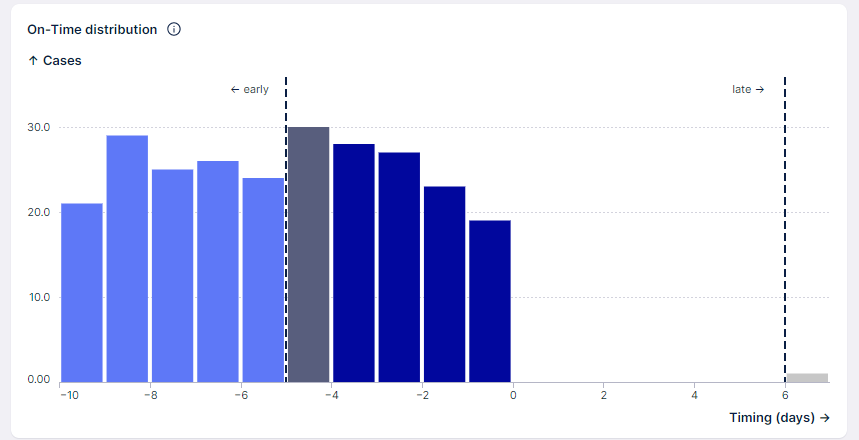
\includegraphics[width=\textwidth]{imgCelonis/SecondaSimulazione/on-time-distribution.png}
    \caption{Grafico di distribuzione dei casi in base al loro completamento rispetto alle scedenze}
    \label{fig:grafico-on-time-distribution}
\end{figure}
\custombold{Assi del grafico}\\
\begin{itemize}
    \item \custombold{Asse Y (Cases)}: rappresenta il numero di casi, con un intervallo che va da 0 a 30;
    \item \custombold{asse X (Timing in days)}: rappresenta i giorni di anticipo o ritardo rispetto alla scadenza. Il lato sinistro dell'asse X indica i giorni di anticipo (early), mentre il lato destro indica i giorni di ritardo (late).
\end{itemize}
\custombold{Barre del grafico}
\begin{itemize}
    \item \custombold{Barre azzurre}: indicano i casi completati in anticipo;
    \item \custombold{barre blu scuro}: indicano i casi completati in tempo;
    \item \custombold{barre grigie}: indicano i casi completati in ritardo.
\end{itemize}
\custombold{Analisi e interpretazione}
Il grafico fornisce una visione dettagliata di come i casi sono distribuiti in relazione al loro completamento anticipato, puntuale o ritardato. Analizzando i dati, emerge che la maggior parte delle attività tende a essere completata in anticipo, con un picco tra i 6 e 8 giorni prima della scadenza, suggerendo una propensione a concludere le attività ben prima del termine previsto.\\
Inoltre, sono presenti diversi casi completati esattamente in tempo, evidenziati dalle barre blu scuro, che indicano una buona gestione delle scadenze per queste attività.\\
Infine, un numero minore di attività risulta completato in ritardo, con alcuni casi che si protraggono fino a 6 giorni dopo la scadenza, evidenziando aree in cui è necessario migliorare il rispetto dei tempi previsti.\\

\custombold{Tasso di puntualità attuale e potenziali aree di miglioramento}\\
Questa schermata fornisce una panoramica del tasso di puntualità attuale e delle potenziali aree di miglioramento.\\
\begin{figure}[H]
    \centering
    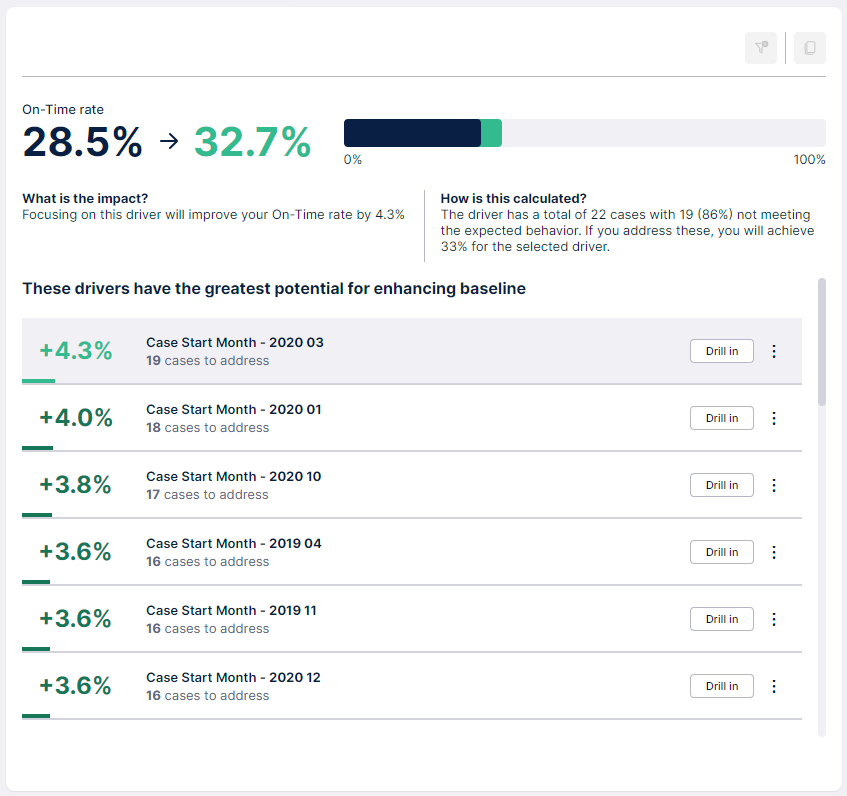
\includegraphics[width=\textwidth]{imgCelonis/SecondaSimulazione/attual-rate-and-improvments.png}
    \caption{Schermata del tasso di puntualità attuale e di possibili miglioramenti}
    \label{fig:grafico-attual-rate-improvments}
\end{figure}
\custombold{On-Time rate}\\
\begin{itemize}
    \item \custombold{On-Time rate}: mostra il tasso di puntualità attuale, che è del 28.5\%;
    \item \custombold{frecce di incremento}: indicano un possibile miglioramento del tasso di puntualità al 32.7\%;
    \item \custombold{barra di progresso}: rappresenta visivamente il miglioramento dal tasso attuale al tasso potenziale.
\end{itemize}
\custombold{Descrizione dell'impatto}\\
\begin{itemize}
    \item \custombold{What is the impact?}: una spiegazione dell'impatto, che indica che concentrarsi su questo driver migliorerà il tasso di puntualità del 4.3\%;
    \item \custombold{How is this calculated?}: una spiegazione del calcolo, indicando che il driver ha un totale di 22 casi con 19 (86\%) che non soddisfano il comportamento previsto. Affrontando questi casi, si raggiungerà un miglioramento del 33\% per il driver selezionato.
\end{itemize}
\custombold{Drivers con maggior potenziale di miglioramento}\\
La sezione inferiore della schermata elenca i drivers (periodi specifici) che hanno il maggiore potenziale per migliorare la baseline del tasso di puntualità.\\
\custombold{Analisi e interpretazione}\\
Questa schermata fornisce una chiara indicazione di dove l'azienda può concentrare gli sforzi per migliorare il tasso di puntualità delle attività. Analizzando i drivers con il maggiore potenziale di miglioramento, le aziende possono identificare i periodi e i casi specifici che contribuiscono maggiormente ai ritardi e pianificare azioni correttive mirate.\\
\subsubsection{Conclusioni}
La funzionalità "Are you meeting the deadlines?" di Celonis rappresenta uno strumento potente per il monitoraggio e l'analisi del rispetto delle scadenze nei processi aziendali. Essa permette alle aziende di configurare le scadenze delle attività basandosi su metriche aziendali specifiche e di visualizzare le performance attraverso grafici e tabelle dettagliate. Questa capacità di configurazione precisa è fondamentale per garantire che le scadenze siano realistiche e adeguate alle esigenze operative.\\
Un vantaggio significativo di questa funzionalità è la sua capacità di fornire un monitoraggio continuo delle prestazioni rispetto alle scadenze. Questo permette alle aziende di reagire tempestivamente ai problemi, identificando le inefficienze. Di conseguenza, le azioni correttive possono essere pianificate e implementate in modo più efficiente, migliorando l'efficienza operativa e riducendo i tempi di ciclo.\\
La possibilità di segmentare i dati e di approfondire i dettagli delle attività attraverso filtri e funzionalità di drill-down è un altro vantaggio significativo. Questa capacità analitica consente di comprendere le cause radice dei ritardi e di pianificare interventi correttivi mirati, ottimizzando l'utilizzo delle risorse. Le aziende possono analizzare i trend di completamento, identificando se le attività tendono ad essere completate in anticipo, in tempo o in ritardo, e in che misura. Questo livello di dettaglio analitico è fondamentale per migliorare la gestione del tempo e delle risorse.\\
Tuttavia, ci sono anche alcuni svantaggi da considerare. La configurazione iniziale delle scadenze richiede un'attenzione dettagliata e una comprensione approfondita delle metriche aziendali rilevanti. Se le scadenze non sono impostate correttamente, l'analisi risultante potrebbe essere inaccurata o fuorviante. Inoltre, l'implementazione di azioni correttive basate sui dati richiede un impegno costante da parte dei vari team e dipartimenti, il che può comportare un utilizzo significativo di risorse e tempo. Senza un monitoraggio continuo e un feedback regolare, i miglioramenti potrebbero non essere sostenibili nel lungo termine.

\subsection{Terza simulazione}
Il file CSV è stato creato mediante uno script Python che simula una serie di attività relative alla produzione e alla gestione degli ordini di prodotti. Inoltre, per la simulazione dei dati, sono stati presi in considerazione anche i dati estratti manualmente da un database di un sistema gestionale.
\subsubsection{Regole di simulazione}
\custombold{Impostazione delle date iniziali}\\
Ogni ciclo di attività inizia con la prima attività programmata tra il 1 gennaio 2019 e il 31 dicembre 2020.\\
\custombold{Definizione delle tipologie di prodotti}\\
Viene creata una lista di 30 tipi di scarpe, denominate "Scarpe tipo 1" fino a "Scarpe tipo 30".\\
\custombold{Definizione delle attività e delle durate}\\
Sono state definite 17 attività, ciascuna con un ID unico e una durata variabile. Le durate delle attività sono espresse in minuti o giorni, a seconda dell'attività specifica.\\
\custombold{Generazione di un ciclo di attività per prodotto}\\
Per ciascun prodotto, viene generato un ciclo di attività che segue le seguenti regole:
\begin{itemize}
    \item \custombold{attività obbligatorie}: alcune attività avvengono in un ordine fisso. Ad esempio, "Conferma ordine" è sempre seguita da "Creazione progetto";
    \item \custombold{modifica del progetto}: un numero casuale di modifiche al progetto (da 1 a 5) può essere aggiunto dopo la creazione del progetto;
    \item \custombold{gestione degli ordini fornitore}: un numero casuale (da 1 a 3) di cicli di gestione ordini fornitore può essere inserito, ognuno dei quali può includere attività come "Ordine fornitore", "Arrivo offerta fornitore", "Ordine annullato" o "Ordine sospeso";
    \item \custombold{produzione}: vengono aggiunte attività relative alla produzione, come "Stampa scheda di produzione", "Inizio ciclo di produzione" e "Termine ordine di produzione";
    \item \custombold{attività non necessarie}: possono essere inserite attività opzionali come "Controllo qualità non necessario" (20\% di probabilità) e "Ri-lavorazione non necessaria" (10\% di probabilità);
    \item \custombold{consegna}: dopo la produzione, viene aggiunta l'attività di "Consegna".
\end{itemize}
\custombold{Generazione dei timestamp}\\
Ogni attività riceve un timestamp generato casualmente basato su un intervallo di tempo definito per quella specifica attività.\\
\custombold{Ciclo di generazione dei dati}\\
Il numero di prodotti varia tra 300 e 500, determinato casualmente. Per ogni prodotto, viene generato un ciclo di attività completo, assicurandosi che tutte le attività obbligatorie siano inserite nel corretto ordine e che le attività casuali siano distribuite come specificato.\\
\custombold{Mischiamento casuale delle righe del file CSV}\\
È stato utilizzato un algoritmo per mischiare in modo casuale le righe del file CSV. L'algoritmo legge il file CSV originale e separa l'intestazione dai dati. Successivamente, le righe dei dati vengono mescolate casualmente mantenendo intatta l'intestazione. Infine, il nuovo file CSV, con le righe mescolate, viene salvato in un file di output. Questo processo assicura che i dati siano riorganizzati in modo casuale senza alterare la struttura del file CSV.

\subsubsection{Analisi delle attività non desiderate}
La funzionalità di analisi delle attività non desiderate di Celonis è uno strumento utile per identificare e analizzare le attività indesiderate all'interno di un processo aziendale. Questa esplorazione aiuta le aziende a individuare le inefficienze e i passaggi non necessari che possono essere eliminati o ottimizzati.\\
\custombold{Configurazione}\\
Questa sezione invita l'utente a selezionare le attività che non dovrebbero verificarsi nel processo. Le attività indesiderate possono includere blocchi, modifiche o altre attività che rallentano il processo o lo rendono inefficiente.
\begin{figure}[H]
    \centering
    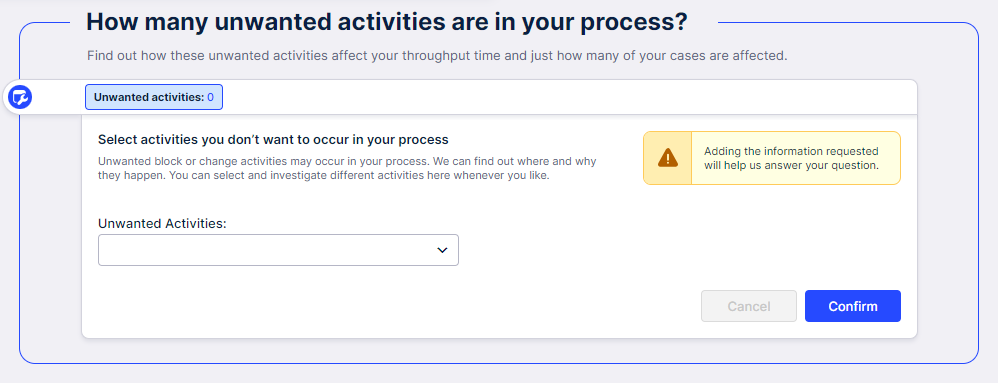
\includegraphics[width=\textwidth]{imgCelonis/TerzaSimulazione/unwanted-activities-configuration.png}
    \caption{Schermata di configurazione dell'analisi delle attività indesiderate}
    \label{fig:configurazione-unwanted-activities}
\end{figure}
\custombold{Campo di selezione}\\
\begin{itemize}
    \item \custombold{Unwanted activities}: un menu a tendina che permette di selezionare le attività specifiche che si considerano indesiderate. Selezionando un'attività dal menu, è possibile investigare dove e perché queste attività si verificano nel processo.
\end{itemize}

\custombold{Unwanted activity rate}\\
Questa schermata fornisce informazioni chiave sul tasso di attività indesiderate e il loro impatto sui tempi di ciclo del processo.\\
\begin{figure}[H]
    \centering
    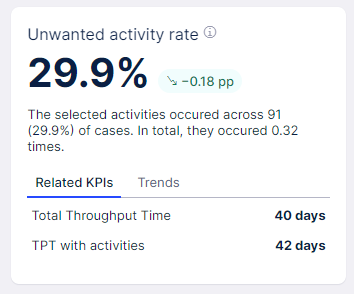
\includegraphics[width=\textwidth]{imgCelonis/TerzaSimulazione/unwanted-activity-rate.png}
    \caption{Schermata di monitoraggio del tasso di attività indesiderate}
    \label{fig:schermata-unwanted-activity-rate}
\end{figure}
\custombold{Dettagli delle attività indesiderate}\\
In questo caso le attività indesiderate selezionate si sono verificate in 91 casi su 303 totali, pari al 29.9\% del totale analizzato. In media, queste attività si sono verificate 0.32 volte per caso.\\
\custombold{Indicatori di performance collegati}\\
\begin{itemize}
    \item \custombold{Total throughput time}: il tempo totale di completamento del processo senza considerare le attività indesiderate, che è di 40 giorni;
    \item \custombold{TPT with activities}: il tempo totale di completamento del processo considerando le attività indesiderate, che è di 42 giorni, suggerendo che la presenza di attività indesiderate aggiunge 2 giorni al tempo totale di completamento del processo.
\end{itemize}
\custombold{Analisi e interpretazione}\\
Questa schermata offre una visione chiara dell'impatto delle attività indesiderate sui processi aziendali. Il tasso di attività indesiderate del 29.9\% indica che queste attività si verificano con una certa frequenza, influenzando negativamente l'efficienza del processo. La diminuzione del tasso di attività indesiderate di 0.18 punti percentuali è un segnale positivo di miglioramento.\\
Il confronto tra il "Total Throughput Time" (40 giorni) e il "TPT with activities" (42 giorni) evidenzia che le attività indesiderate aumentano il tempo di completamento del processo di 2 giorni.\\

\custombold{Activity frequency}\\
Il grafico mostra quante volte ciascuna attività indesiderata si è verificata.\\
\begin{figure}[H]
    \centering
    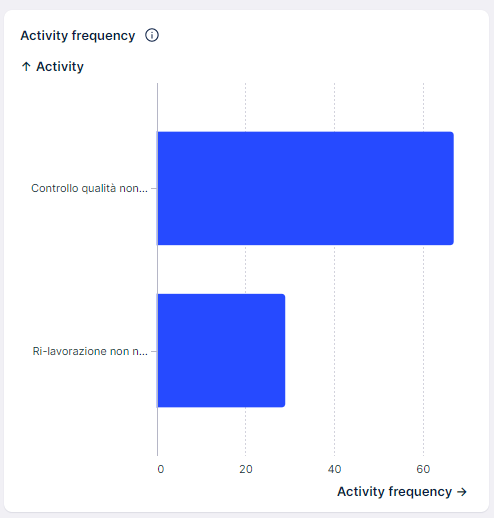
\includegraphics[width=\textwidth]{imgCelonis/TerzaSimulazione/activity-frequency.png}
    \caption{Grafico della frequenza delle attività indesiderate}
    \label{fig:grafico-activity-frequency}
\end{figure}
\custombold{Barre del grafico}\\
Il grafico è costituito da due barre, ciascuna rappresentante una diversa attività indesiderata:
\begin{itemize}
    \item \custombold{barra superiore}: rappresenta la frequenza con cui si verifica l'attività "Controllo qualità non necessario";
    \item \custombold{barra inferiore}: rappresenta la frequenza con cui si verifica l'attività "Ri-lavorazione non necessaria".
\end{itemize}
\custombold{Dati specifici}\\
\begin{itemize}
    \item \custombold{Controllo qualità non necessario}: questa attività si è verificata circa 60 volte, indicando che il controllo qualità è stato eseguito in situazioni dove non era richiesto;
    \item \custombold{Ri-lavorazione non necessaria}: questa attività si è verificata circa 30 volte, mostrando che la ri-lavorazione è stata eseguita più frequentemente del necessario.
\end{itemize}
\custombold{Interpretazione del grafico}\\
Il grafico offre una rappresentazione chiara e sintetica della frequenza delle attività indesiderate all'interno del processo. La sua suddivisione in due sezioni permette di comprendere rapidamente quale attività si verifica più frequentemente e con quale frequenza.\\
Un elemento significativo emerso dall'analisi è l'elevata frequenza del "Controllo qualità non necessario", con circa 60 occorrenze. Questo dato suggerisce che c'è un problema rilevante legato all'esecuzione di controlli qualità non necessari, che potrebbero essere eliminati o ridotti per migliorare l'efficienza del processo.\\
La "Ri-lavorazione non necessaria" si verifica meno frequentemente, con circa 30 occorrenze, ma rappresenta comunque un'opportunità per ottimizzare il processo. Ridurre la necessità di ri-lavorazione potrebbe migliorare il flusso di lavoro e ridurre i tempi di ciclo complessivi.\\

\custombold{Occurrence per case affected}\\
Il grafico mostra quante volte le attività indesiderate si verificano in media per caso.\\
\begin{figure}[H]
    \centering
    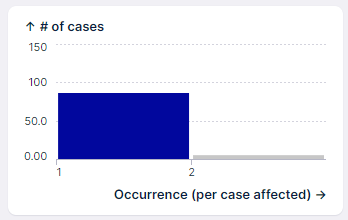
\includegraphics[width=\textwidth]{imgCelonis/TerzaSimulazione/occurrence-per-case-affected.png}
    \caption{Grafico della frequenza delle occorrenze per caso influenzato nel processo}
    \label{fig:grafico-occurrence-per-case-affected}
\end{figure}
\custombold{Barre del grafico}\\
Il grafico è costituito da due barre di colori diversi, ciascuna rappresentante una diversa occorrenza per caso influenzato:
\begin{itemize}
    \item \custombold{barra blu}: rappresenta il numero di casi in cui le attività indesiderate si sono verificate una volta per caso;
    \item \custombold{barra grigia}: rappresenta il numero di casi in cui le attività indesiderate si sono verificate due volte per caso.
\end{itemize}
\custombold{Dati specifici}\\
\begin{itemize}
    \item \custombold{Occorrenza singola}: la barra blu mostra che 86 casi hanno avuto un'attività indesiderata verificata una sola volta;
    \item \custombold{occorrenza doppia}: la barra grigia mostra che ci sono 5 casi in cui le attività indesiderate si sono verificate due volte per caso.
\end{itemize}
\custombold{Interpretazione del grafico}\\
Il grafico offre una rappresentazione chiara e sintetica della frequenza con cui le attività indesiderate si verificano per caso. La sua suddivisione in due sezioni permette di comprendere rapidamente quanti casi sono stati influenzati dalle attività indesiderate e con quale frequenza.\\
Un elemento significativo emerso dall'analisi è che la maggior parte dei casi influenzati dalle attività indesiderate ha subito tali attività una sola volta per caso. Questo suggerisce che, sebbene le attività indesiderate siano presenti, tendono a non ripetersi frequentemente nello stesso caso.\\

\custombold{Unwanted activities per case over time}\\
Il grafico mostra il numero di casi totali e i casi con attività indesiderate per ciascun mese.\\
\begin{figure}[H]
    \centering
    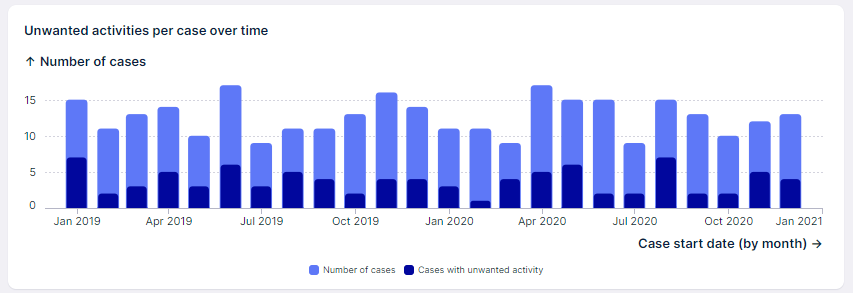
\includegraphics[width=\textwidth]{imgCelonis/TerzaSimulazione/unwanted-activities-per-case-over-time.png}
    \caption{Grafico della frequenza delle attività indesiderate per caso nel tempo}
    \label{fig:grafico-unwanted-activities-per-case-over-time}
\end{figure}
\custombold{Barre del grafico}\\
Il grafico è costituito da due tipi di barre colorate, ciascuna rappresentante una diversa categoria di casi:\\
\begin{itemize}
    \item \custombold{barre azzurre}: rappresentano il numero totale di casi per ogni mese;
    \item \custombold{barre blu}: rappresentano il numero di casi che includono attività indesiderate per ogni mese.
\end{itemize}
\custombold{Dati specifici}\\
\begin{itemize}
    \item \custombold{Numero totale di casi}: le barre azzurre mostrano il numero totale di casi iniziati ogni mese, che varia tra circa 10 e 15 casi al mese;
    \item \custombold{casi con attività indesiderate}: le barre blu mostrano il numero di casi con attività indesiderate, che varia tra circa 2 e 7 casi al mese.
\end{itemize}
\custombold{Interpretazione del grafico}\\
Il grafico offre una rappresentazione chiara e sintetica della frequenza delle attività indesiderate per caso nel tempo. La sua suddivisione in due categorie di barre permette di comprendere rapidamente la proporzione di casi totali che includono attività indesiderate in ciascun mese.\\
Un elemento significativo emerso dall'analisi è che, sebbene il numero totale di casi per mese rimanga relativamente costante, la proporzione di casi con attività indesiderate varia. Ad esempio, nei mesi di luglio 2019 e aprile 2020, si osserva un numero relativamente alto di casi totali e anche un numero significativo di casi con attività indesiderate. Questo potrebbe indicare periodi specifici in cui le inefficienze del processo erano più prevalenti.\\

\custombold{Unwanted activities rate breakdown}\\
Questa tabella offre una suddivisione dettagliata del tasso di attività indesiderate per mese di inizio dei casi analizzati.\\
\begin{figure}[H]
    \centering
    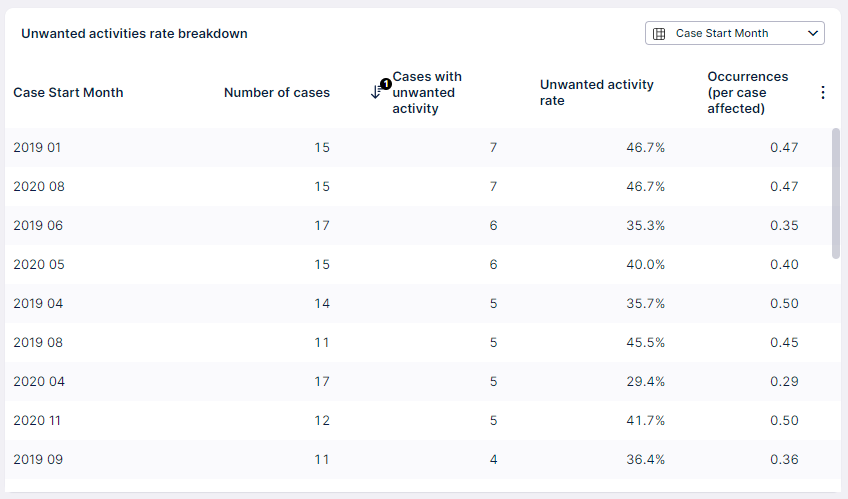
\includegraphics[width=\textwidth]{imgCelonis/TerzaSimulazione/unwanted-activities-rate-breakdown.png}
    \caption{Tabella del tasso di attività indesiderate per mese di inizio}
    \label{fig:tabella-unwanted-activities-rate-breakdown}
\end{figure}
\custombold{Intestazione delle colonne}\\
\begin{itemize}
    \item \custombold{Case start month}: il mese di inizio dei casi analizzati;
    \item \custombold{Number of cases}: il numero di casi iniziati in quel mese specifico;
    \item \custombold{Cases with unwanted activity}: il numero di casi che includono attività indesiderate;
    \item \custombold{Unwanted activity rate}: la percentuale di casi con attività indesiderate rispetto al totale dei casi per quel mese;
    \item \custombold{Occurrences (per case affected)}: il numero medio di occorrenze di attività indesiderate per ciascun caso influenzato.
\end{itemize}
\custombold{Interpretazione della tabella}\\
La tabella offre una visione dettagliata di come le attività indesiderate influenzano i processi nei diversi mesi. Permette di identificare i periodi con la maggiore incidenza di attività indesiderate, evidenziando i mesi in cui l'efficienza del processo è più compromessa.\\

\custombold{Tasso di attività indesiderate attuale e potenziali aree di miglioramento}\\
Questa schermata fornisce una panoramica del tasso di attività indesiderate attuale e delle potenziali aree di miglioramento.\\
\begin{figure}[H]
    \centering
    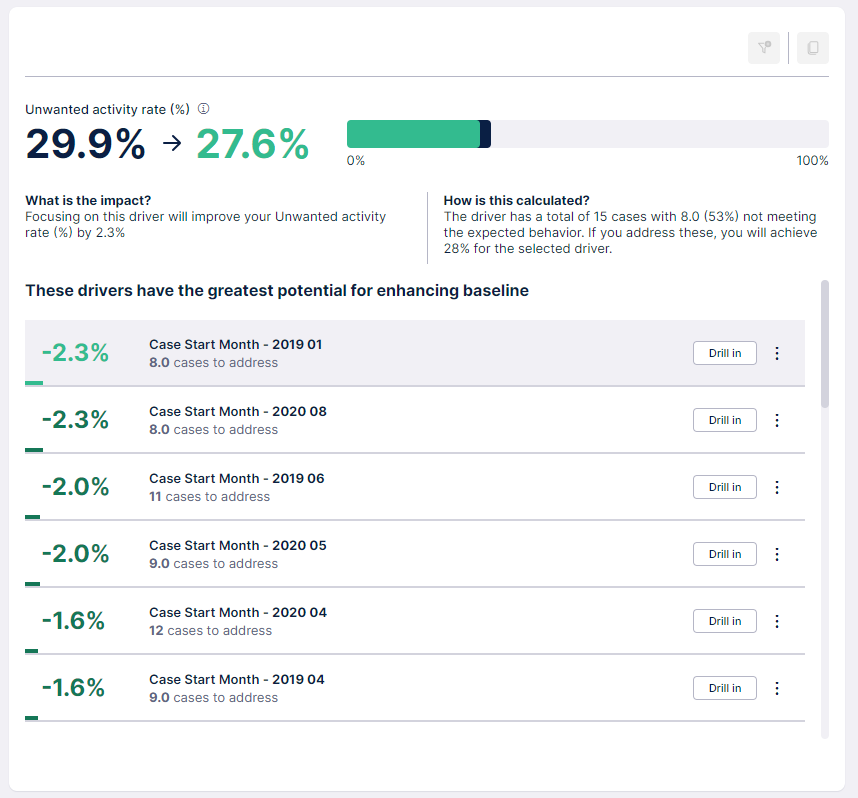
\includegraphics[width=\textwidth]{imgCelonis/TerzaSimulazione/unwanted-rate-and-improvments.png}
    \caption{Schermata del tasso di attività indesiderate e dei potenziali miglioramenti}
    \label{fig:schermata-unwanted-rate-and-improvments}
\end{figure}
\custombold{Unwanted activity rate}\\
\begin{itemize}
    \item \custombold{Unwanted activity rate}: mostra il tasso di attività indesiderate attuale, che è del 29.9\%;
    \item \custombold{frecce di decremento}: indicano un possibile miglioramento del tasso di attività indesiderate al 27.6\%;
    \item \custombold{barra di progresso}: rappresenta visivamente il miglioramento dal tasso attuale al tasso potenziale;
\end{itemize}
\custombold{Descrizione dell'impatto}\\
\begin{itemize}
    \item \custombold{What is the impact?}: una spiegazione dell'impatto, che indica che concentrarsi su questo driver migliorerà il tasso di attività indesiderate del 2.3\%;
    \item \custombold{How is this calculated?}: una spiegazione del calcolo, indicando che il driver ha un totale di 15 casi con 8 (53\%) che non soddisfano il comportamento previsto. Affrontando questi casi, si raggiungerà un miglioramento del 28\% per il driver selezionato;
\end{itemize}
\custombold{Drivers con maggior potenziale di miglioramento}\\
La sezione inferiore della schermata elenca i drivers (periodi specifici) che hanno il maggiore potenziale per migliorare la baseline del tasso di attività indesiderate.\\
\custombold{Analisi e interpetazione}\\
Questa schermata fornisce una chiara indicazione di dove l'azienda può concentrare gli sforzi per migliorare il tasso di attività indesiderate. Analizzando i drivers con il maggiore potenziale di miglioramento, le aziende possono identificare i periodi e i casi specifici che contribuiscono maggiormente alle attività indesiderate e pianificare azioni correttive mirate.\\
Concentrarsi sui mesi con i maggiori potenziali di miglioramento, come gennaio 2019 e agosto 2020, dove si possono migliorare i tassi di attività indesiderate del 2.3\%, permette di implementare strategie mirate per ridurre significativamente le inefficienze.\\
\subsubsection{Conclusioni}
La funzionalità di analisi delle attività non desiderate di Celonis rappresenta uno strumento prezioso per le aziende che desiderano ottimizzare i loro processi aziendali eliminando inefficienze e passaggi non necessari. Attraverso la configurazione personalizzata, gli utenti possono identificare attività specifiche che rallentano il processo, come blocchi o modifiche inutili. I dati raccolti mostrano che le attività indesiderate influenzano negativamente il ciclo del processo, aumentando il tempo di completamento da 40 a 42 giorni. Questo impatto è ulteriormente evidenziato dall'analisi della frequenza delle attività indesiderate, che rivela come il "Controllo qualità non necessario" si verifichi circa 60 volte e la "Ri-lavorazione non necessaria" circa 30 volte.\\
La distribuzione delle occorrenze per caso dimostra che, sebbene queste attività tendano a non ripetersi frequentemente nello stesso caso, la loro presenza sporadica è comunque significativa. La variazione mensile dei casi totali e dei casi con attività indesiderate indica periodi specifici in cui le inefficienze sono più pronunciate, suggerendo la necessità di interventi mirati in quei periodi. La tabella del tasso di attività indesiderate fornisce una visione dettagliata delle incidenze mensili, facilitando l'identificazione dei mesi con la maggiore incidenza di attività indesiderate.\\
Infine, la schermata che illustra il tasso di attività indesiderate e le potenziali aree di miglioramento offre una panoramica chiara delle opportunità di ottimizzazione. Con un tasso attuale del 29.9\%, la possibilità di miglioramento fino al 27.6\% rappresenta un obiettivo concreto per le aziende. Concentrarsi sui periodi con il maggior potenziale di miglioramento permette di pianificare azioni correttive mirate, riducendo significativamente le inefficienze e migliorando l'efficienza complessiva del processo aziendale.
\end{document}
